\section{Анализ деятельности ООО \enquote{Сампад} в области разработки программного обеспечения для сферы Интернета вещей}
\label{sec:analysis}

\subsection{Общая характеристика и основные направления деятельности ООО \enquote{Сампад}}
\label{sec:develop:company}

Компания Sampad основана в 2013 году. Полное название предприятия: общество с ограниченной ответственностью \enquote{Сампад}. Компания является разработчиком заказного программного обеспечения и поставщиком ИТ-услуг  для компаний из различных стран. Штаб-квартира компании расположена в Минске, также есть офис в США. Штат сотрудников насчитывает более 80 инженеров и IT-консультантов \cite{sampad_data}.
Sampad имеет большой опыт в таких областях, как:
\begin{itemize}
    \item нативные мобильные приложения (iOS: Obj C/Swift, Android: Java/Kotlin);
    \item кроссплатформенные мобильные приложения (React Native, Cordova Ionic, Flutter);
    \item финансовые бизнес-приложения, Fintech (Python, ASP .Net);
    \item IoT приложения;
    \item поддержка бизнес-приложений.
\end{itemize}
Преимуществами сотрудничества с Sampad пользуются десятки компаний из различных секторов экономики, в том числе:

\begin{itemize}
    \item банки и финансовые компании;
    \item розничная торговля и потребительские товары;
    \item информационный и медиа-бизнес;
    \item индустрия путешествий;
    \item образование;
    \item медицина;
    \item сельское хозяйство;
    \item страхование;
    \item спорт;
    \item рекрутинг;
    \item автобизнес.
\end{itemize}
Основными заказчиками являются: Microsoft, Oracle, The Coca-Cola Company, McDonalds, Nestle, Timotei и многие другие.

Компания делает большой акцент на проектах с использованием искусственного интеллекта (машинное обучение, нейронные сети и др.). Существуют проекты в сфере образования, сбора финансовой информации, кредитования малого и среднего бизнеса, а также приложения для сельского хозяйства (предсказание появления насекомых на полях).

\subsection{Деятельность ООО \enquote{Сампад} в сфере Интернета вещей}
\label{sec:develop:companyGarlands}

Индустрия электронного светового оборудования и рынок IoT занимают особое место в деятельности кампании Sampad. Первый проект в данной сфере появился еще в 2016 году. На данный момент существует уже 4 проекта со схожей тематикой и еще несколько находятся на стадии проектирования. Компания разрабатывает как мобильные и веб приложения для управления световым оборудованием, так и прошивку для самого оборудования (C/C++, Arduino). Также компания консультирует заказчиков по поводу электронных компонентов, находящихся в данном оборудовании, хоть и не отвечает непосредственно за разработку электронных схем.

Динамика роста прибыли компании Sampad в сфере Интернета вещей за последний год показывает отличный прогресс (Рисунок \ref{fig:analysis:companyGarlands:sampadIncome}).

~
\begin{figure}[H]
\centering
	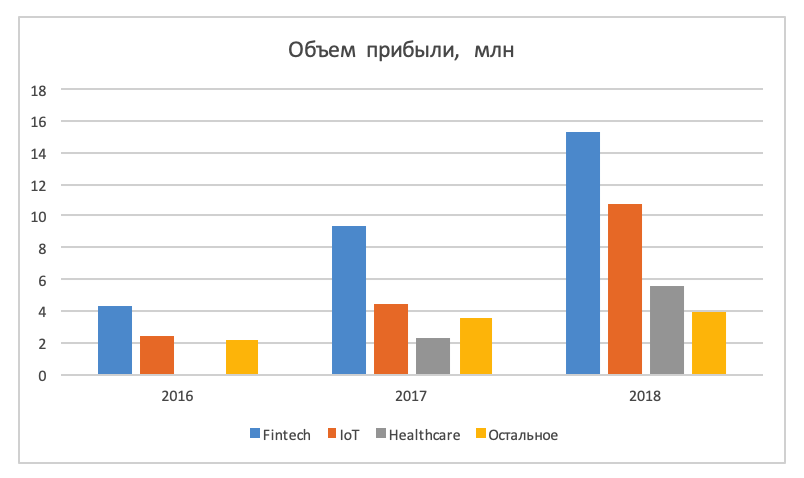
\includegraphics[scale=1]{figures/sampadIncome.png}
	\caption{Прибыль компании Sampad в различных сферах}
	\label{fig:analysis:companyGarlands:sampadIncome}
\end{figure}

Перед началом проекта по управлению адресными светодиодными лентами, было проведено маркетинговое исследование. Данное исследование выявило самую эффективную платформу для разработки приложения~--- мобильные устройства (Рисунок \ref{fig:analysis:companyGarlands:deviceMarket}). Мобильные телефоны имеются практически у каждого человека, так что выбор данной платформы позволяет совершить самый широкий обхват пользователей. Также мобильные устройства отлично подходят для управления различными устройствами в сети, в том числе и адресной светодиодной лентой.

~
\begin{figure}[H]
\centering
	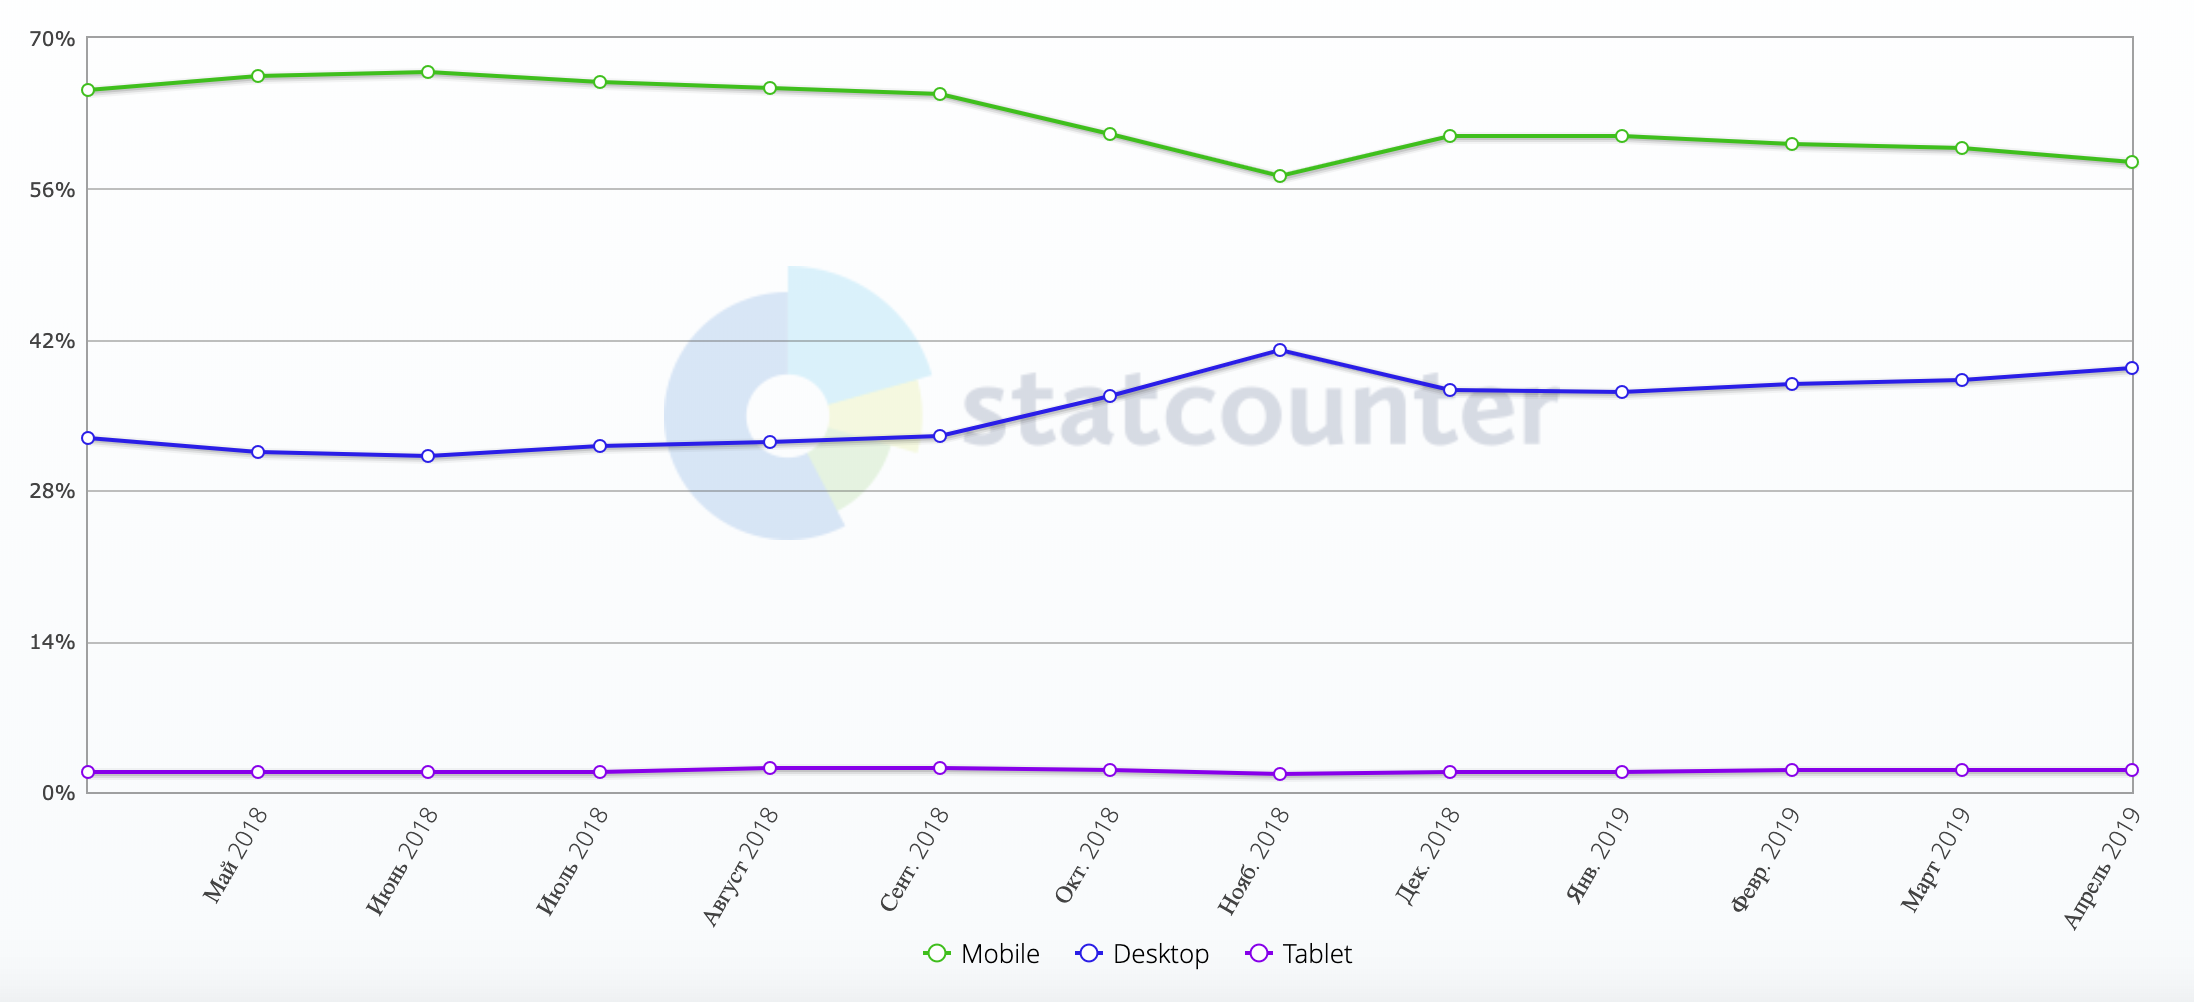
\includegraphics[scale=0.4]{figures/deviceMarket.png}
	\caption{Сравнение количества мобильных устройств, компьютеров и планшетов}
	\label{fig:analysis:companyGarlands:deviceMarket}
\end{figure}

Также были исследованы обе мобильные операционные системы (iOS и Android), и, исходя из полученных данных, было принято решение первоначально сделать приложения для операционной системы Apple iOS (Рисунок \ref{fig:analysis:companyGarlands:digitalMarkets}). Данная операционная система является закрытой и имеет только один, проприетарный магазин приложений. В данных условиях приложение по управлению адресными светодиодными лентами имеет доступ к наиболее полному набору пользователей данной операционной системы.

~
\begin{figure}[H]
\centering
	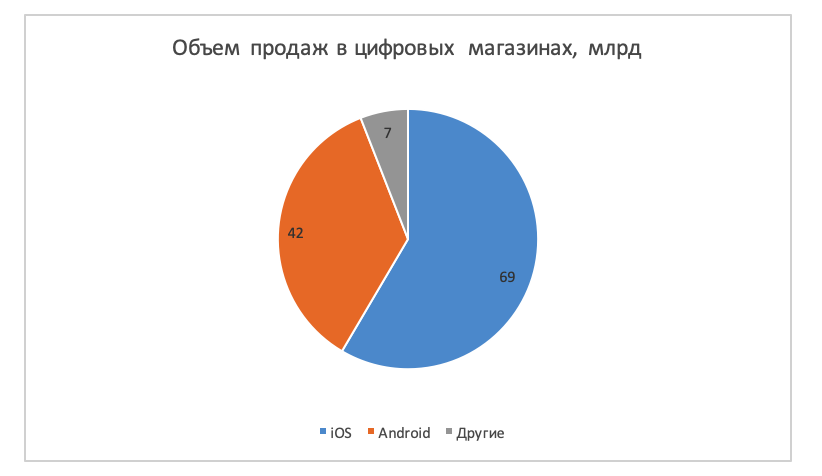
\includegraphics[scale=1]{figures/digitalMarkets.png}
	\caption{Сравнение объема продаж в цифровых магазинах в различных операционных системах}
	\label{fig:analysis:companyGarlands:digitalMarkets}
\end{figure}

По результатам исследования и маркетинговым прогнозам, приложение должно принести большую прибыль компании. Более подробное экономическое обоснование представлено в главе 4.

\subsection{Прогноз и характеристика рынка Интернета вещей в 2019}
\label{sec:analysis:data_art}

В ноябре 2018 года компания DataArt, специализирующаяся на аутсорсинге разработки ПО и таких областях, как интернет-приложения, корпоративные базы данных и инструменты промышленной автоматизации, представила прогноз по развитию рынка интернета вещей в 2019 году.

По словам экспертов, когда-то интернет вещей был нишевой технологией для стартапов, а теперь на ее основе строят бизнес корпорации с оборотом в миллионы долларов. IoT уже изменил жизнь, а 2019 год должен стать периодом значительных перемен в этой области. IoT-специалисты DataArt назвали основные тенденции, которые будут преобладать на рынке интернета вещей в 2019 году.

Устройства станут еще мощнее, обеспечивая локальную обработку данных и возможности искусственного интеллекта. Это уменьшит объемы передачи данных и зависимость от облачных вычислений, а также предоставит больше гибкости компаниям. Граничные вычисления окажут существенное влияние на те отрасли, где необходимо немедленное реагирование, основанное на сложном анализе данных в режиме реального времени (например, производство и общественная безопасность), и там, где облачные коммуникации могут быть ограничены (доставка, логистика и т. п.) \cite{iot_data_2019}.

Ключевым шагом на пути к трансформации отрасли станет гонка компаний, которые будут соперничать в разработке наиболее эффективных и безопасных IoT-решений. Специалисты по IoT-рынку сконцентрируются на решении ключевых проблем безопасности и устранении уязвимостей, связанных с Интернетом вещей, которые прежде препятствовали широкому распространению технологии.

По прогнозам DataArt, в 2019 году будет заметна обостренная конкуренция между технологическими гигантами, вроде Amazon Web Services (AWS), Microsoft и Google, поскольку большие IoT-платформы стали обычным явлением. Такие корпорации смогут захватить большую часть рынка и продолжать расширять зону влияния за счет примыкающих к ним организаций. На фоне борьбы за рыночную долю среди крупных производителей IoT-платформы небольшие компании вынуждены будут для выживания сосредоточиться на нишевых областях (например, перемещение данных, решение специфических проблем в выбранных отраслях, работа с определенными типами устройств и т. д.) \cite{iot_data_2019}.

Аналитики говорят, что в различных отраслях «умные» устройства бесспорно станут еще популярнее. Ожидается растущее использование такой электроники в автомобильном, промышленном, медицинском, производственном и других секторах (Рисунок \ref{fig:analysis:forecast:deviceDiagram}).

~
\begin{figure}[H]
\centering
	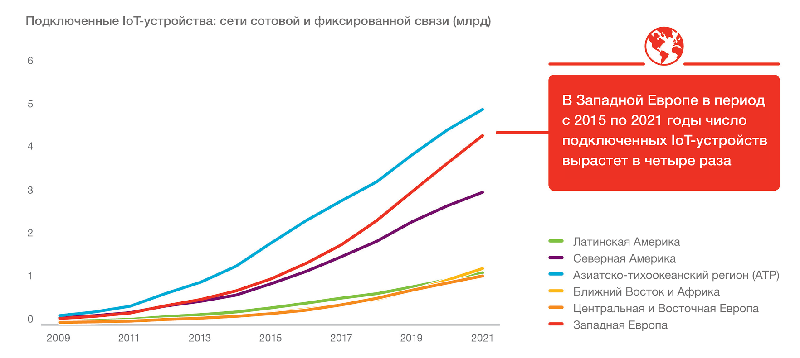
\includegraphics[scale=0.8]{figures/forrester.png}
	\caption{Список подключенных IoT устройств в мире}
	\label{fig:analysis:forecast:deviceDiagram}
\end{figure}

Данные становятся жизненно важной основой автомобильной промышленности. Участники рынка будут и дальше активно внедрять IoT-технологии, чтобы обеспечить машинам незаметный сбор и мониторинг данных, а также их взаимодействие с сервисами «умного» города и другими транспортными средствами.

5G-сети, которые считаются одной из самых ожидаемых технологических тенденций, откроют новую эру для Интернета вещей, способствуя усилению взаимосвязи элементов современного мира. Это приведет к дальнейшему развитию IoT-инноваций, что даст возможность собирать данные, анализировать их и управлять ими практически в режиме реального времени \cite{iot_data_2019}.

Число вендоров, стремящихся занять часть рынка IIoT, продолжает расти, но некоторые лидеры вышли из поля, говорится в другом исследовании. Согласно отчету Forrester Research о программных платформах IIoT, C3 IoT, Microsoft, PTC, SAP и IBM являются лидерами отрасли, при этом самое сильное предложение делает C3 IoT, а IBM намного опережает других поставщиков по стратегии. Amazon Web Services считается только «претендентом» на пространство IIoT, оставшись позади сильнейших игроков, таких как GE, Oracle и Siemens. Forrester поставила Cisco на последнее, 15-е место среди компаний по ассортименту и стратегии. Вендоры оценивались по 24 критериям, включая аналитические возможности, использование технологии цифровых двойников и производственную интеграцию \cite{iot_data_2019}.

Эксперты говорят, что в предыдущие годы эта технология быстро развивалась благодаря широкому распространению сенсоров, а также инфраструктур облачных и периферийных вычислений. В результате интернет вещей стал менять не только бизнес компаний, но и жизнь обычных людей.

В Forrester считают, что концепция централизованного «умного» дома, в котором устройства тесно взаимодействуют между собой, стала мечтой скорее компаний, чем потребителей. Интерес к рынку оборудования для «умных» домов снижается со стороны домашних пользователей, которые предпочитают покупать только одно многофункциональное устройство, управляемое при помощи приложения. Такая тенденция, скорее всего, сохранится в 2019 году. Но компании могут попытаться объединять услуги в пакеты и привлекать клиентов скидками, но люди пока не готовы к такого рода интегрированным коммуникациями, говорится в докладе, выпущенном в ноябре 2018 года \cite{iot_data_2019}.

По словам аналитиков, разговоры об интернете вещей как о непонятном модном термине уйдут на второй план, а на первом — появятся проекты реального применения технологии.

Аналитики считают, что в 2019 году разработчики IoT-платформ будут сужать сферу своей деятельности, сосредотачиваясь на определенных вариантах использования. Например, бизнесменам не нужна одна единственная платформа промышленного интернета вещей для управления каждым процессом в своей компании. Вместо этого они ищут решения, специализирующиеся на конкретных задачах. В связи с этим в 2019 году стоит ожидать еще больше партнерских соглашений с IoT-вендорами.

Еще одним трендом 2019 года эксперты называют кибератаки на системы «умных» городов. Многие города не в состоянии обеспечить безопасность подключенных устройств, датчиков и инфраструктуры связи, а также конфиденциальность граждан в системах умного города. Специалисты прогнозируют увеличение числа целенаправленных атак с помощью программ-вымогателей против уязвимых компонентов развертывания интеллектуальных городов, что приведет к сбоям в обслуживании граждан и заставит города вкладываться в кибербезопасность, чтобы свести к минимуму риск дальнейших атак \cite{iot_data_2019}.

В Forrester видят зарождение рынка услуг по управлению и эксплуатации фрагментированных IoT-объектов.

\subsection{Описание процесса управления адресной светодиодной лентой}
\label{sec:analysis:businessProccess}

Для того, чтобы воспользоваться всеми возможностями адресной светодиодной ленты, пользователь должен первоначально купить ее, установить ее в удобном месте, скачать описанное в записке программное обеспечение на мобильный телефон и провести процесс инициализации адресной ленты.

Функционирование украшения дома в данном проекте описаны с помощью функциональной модели IDEF0.

Для представления процессов, возникающих при приобретении и использовании адресных светодиодных лент (украшений) была разработана функциональная модель \enquote{Управлять адресной светодиодной лентой}. Процесс состоит из нескольких этапов, которые подробно описаны на рисунках~\ref{fig:analysis:functionalModel:main}~–~\ref{fig:analysis:functionalModel:a42_connecting}.

~
\begin{figure}[H]
\centering
	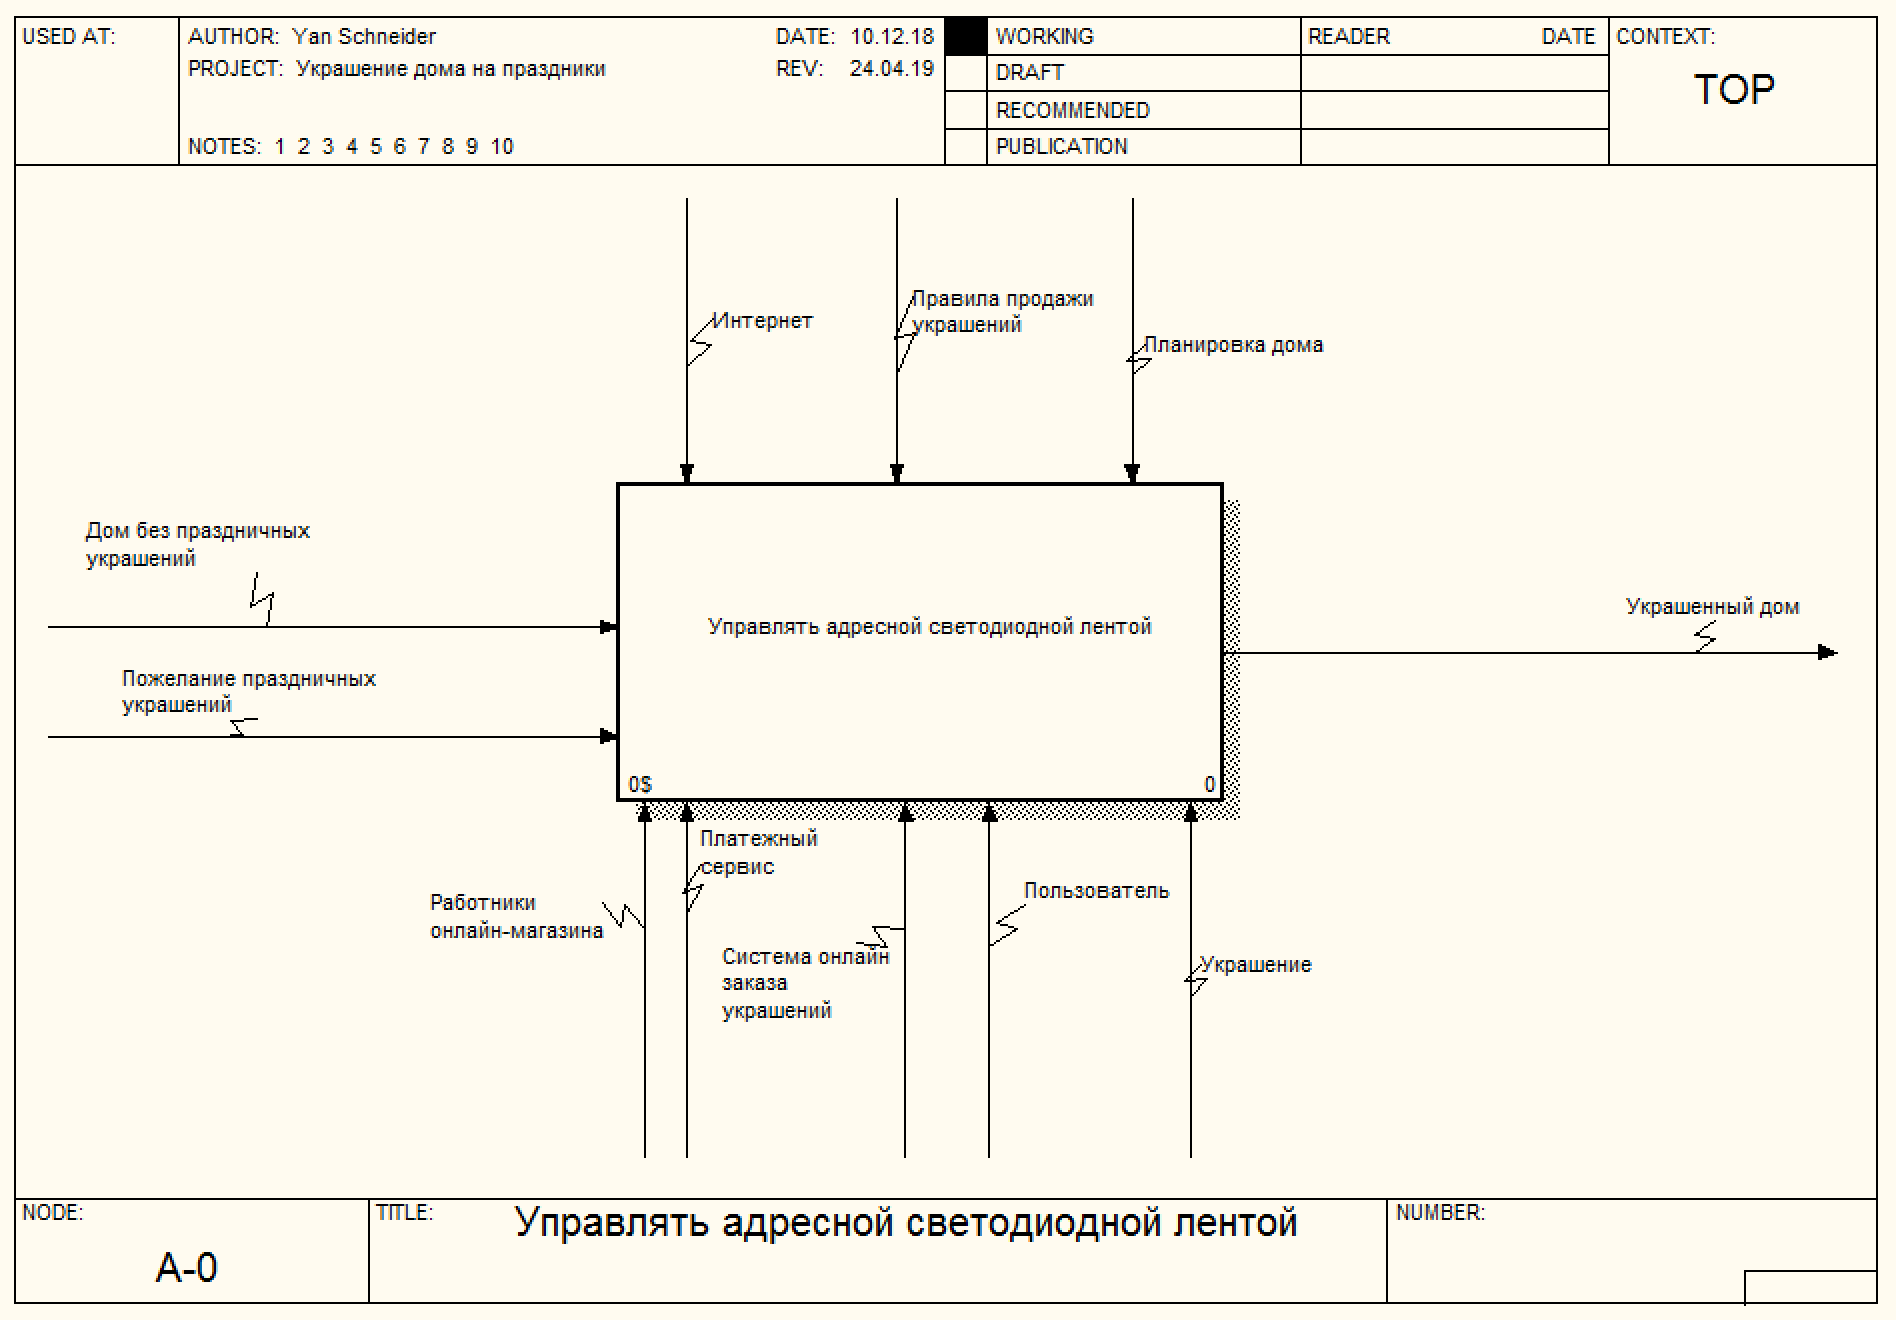
\includegraphics[scale=0.45]{figures/functionalModel/main.png}
	\caption{Контекстная диаграмма процесса управления адресной светодиодной лентой}
	\label{fig:analysis:functionalModel:main}
\end{figure}

На рисунке~\ref{fig:analysis:functionalModel:main} представлена контекстная диаграмма верхнего уровня, входными данными для которой являются дом без украшений и пожелания к ним. В рамках процесса на выходе получается украшенный дом. 

К механизмам управления относятся Интернет, правила продажи украшений и планировка дома пользователя.

Механизмы, осуществляющие процесс: работник онлайн-магазина, платежный сервис, система онлайн-заказа украшений, пользователь и само украшение (адресная светодиодная лента).

Далее в соответствии со вторым и третьим принципами, распишем основное действие на уровни.

Украшение дома декомпозировано на 4 блока: поиск, покупка, установка и настройка украшений.

Функциональная модель управления адресной светодиодной лентой показана на рисунке~\ref{fig:analysis:functionalModel:a0_decoration}.

~
\begin{figure}[H]
\centering
	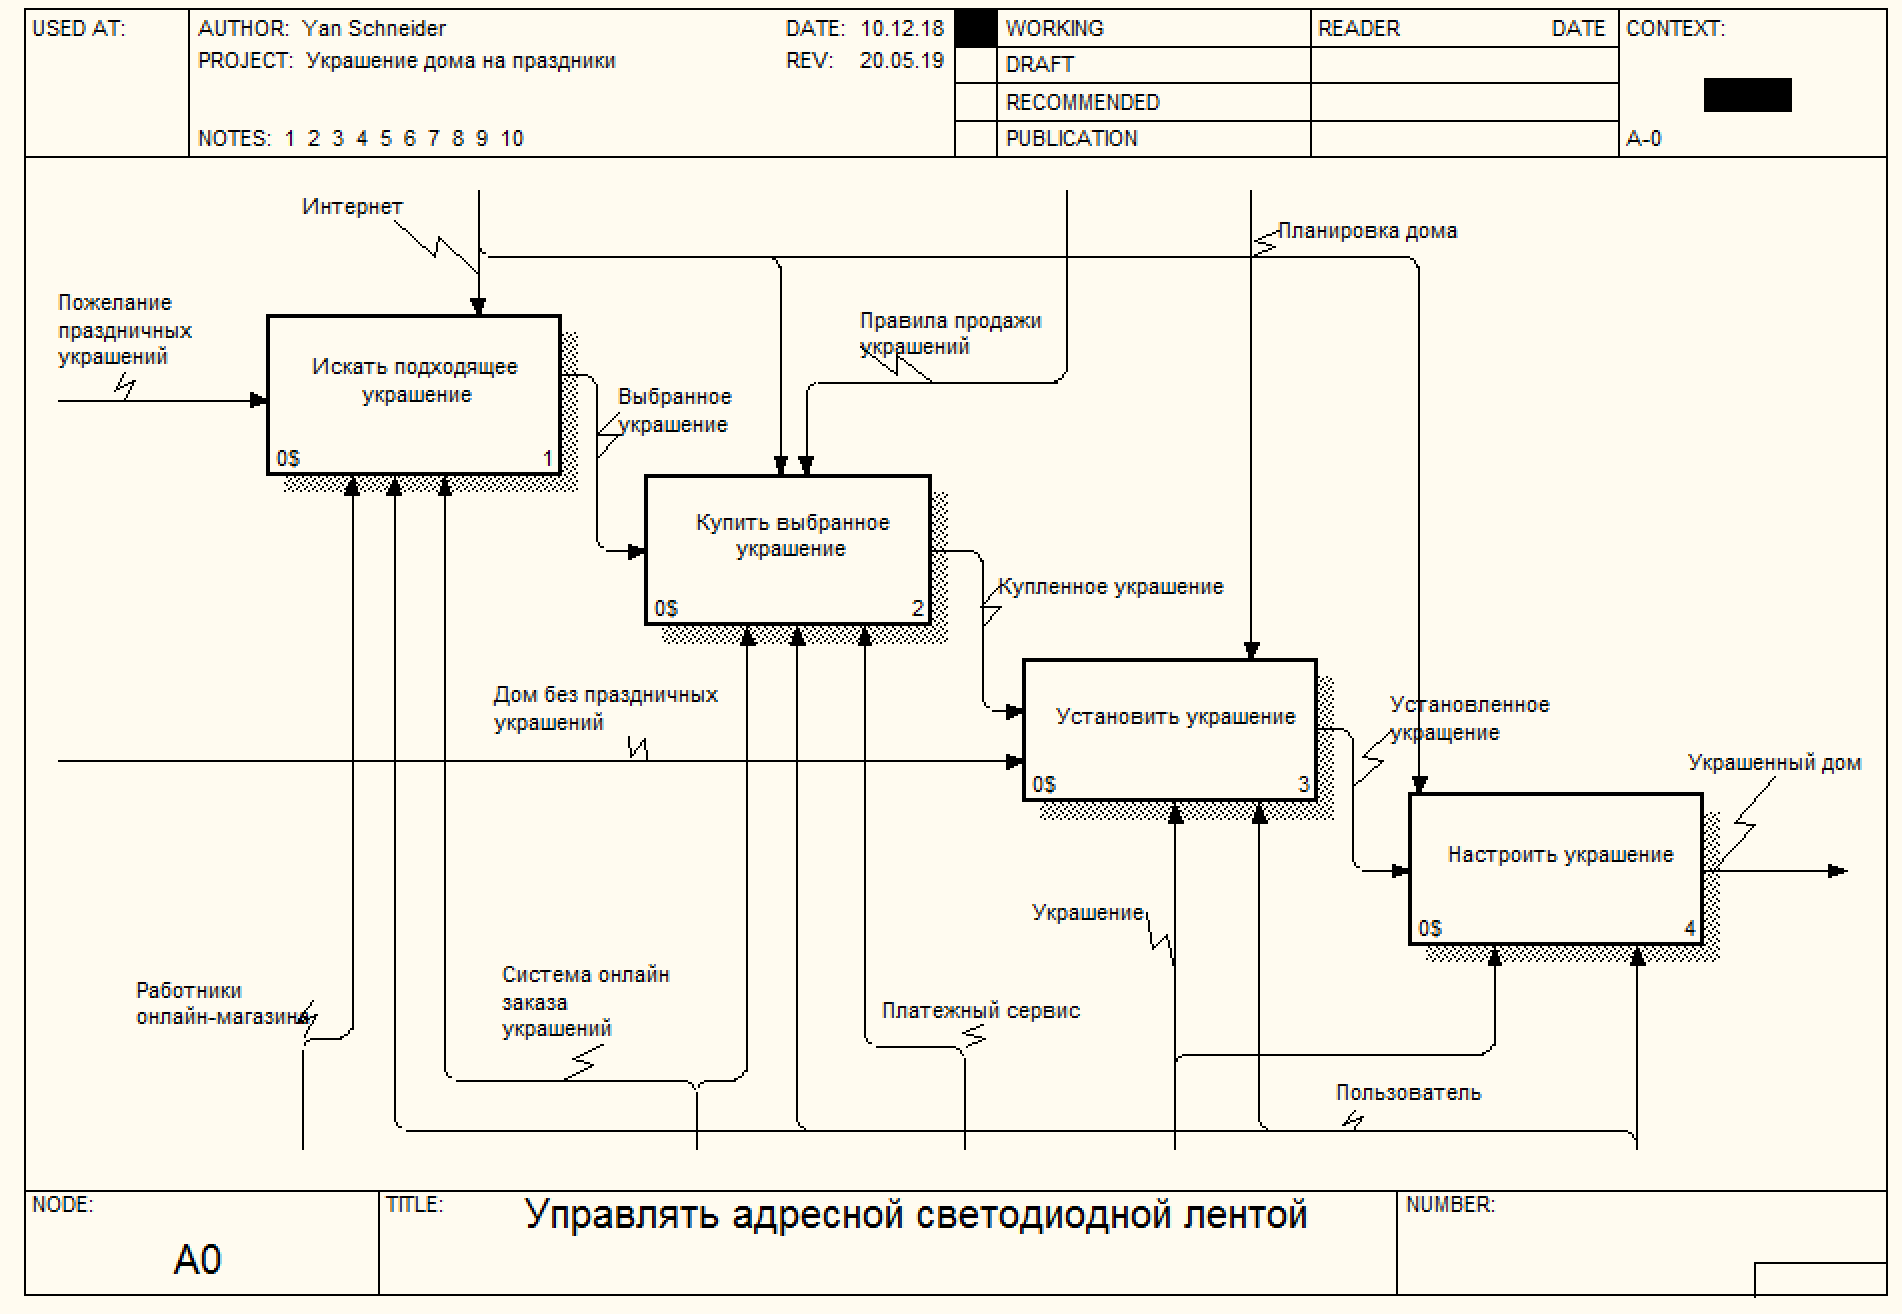
\includegraphics[scale=0.45]{figures/functionalModel/a0_decoration.png}
	\caption{Декомпозиция блока \enquote{Управлять адресной светодиодной лентой}}
	\label{fig:analysis:functionalModel:a0_decoration}
\end{figure}

Рассмотрим последовательно каждый блок.

Первый блок (рисунок~\ref{fig:analysis:functionalModel:a1_search}):

Данный блок необходим для поиска подходящего украшения для дома. Данный процесс включает в себя вход в онлайн магазин, установку фильтров для поиска, просмотр результатов поиска, консультация с работником онлайн-магазина (для дополнительной фильтрации списка выбранных украшений) и, наконец, выбор подходящего варианта.

 ~
\begin{figure}[H]
\centering
	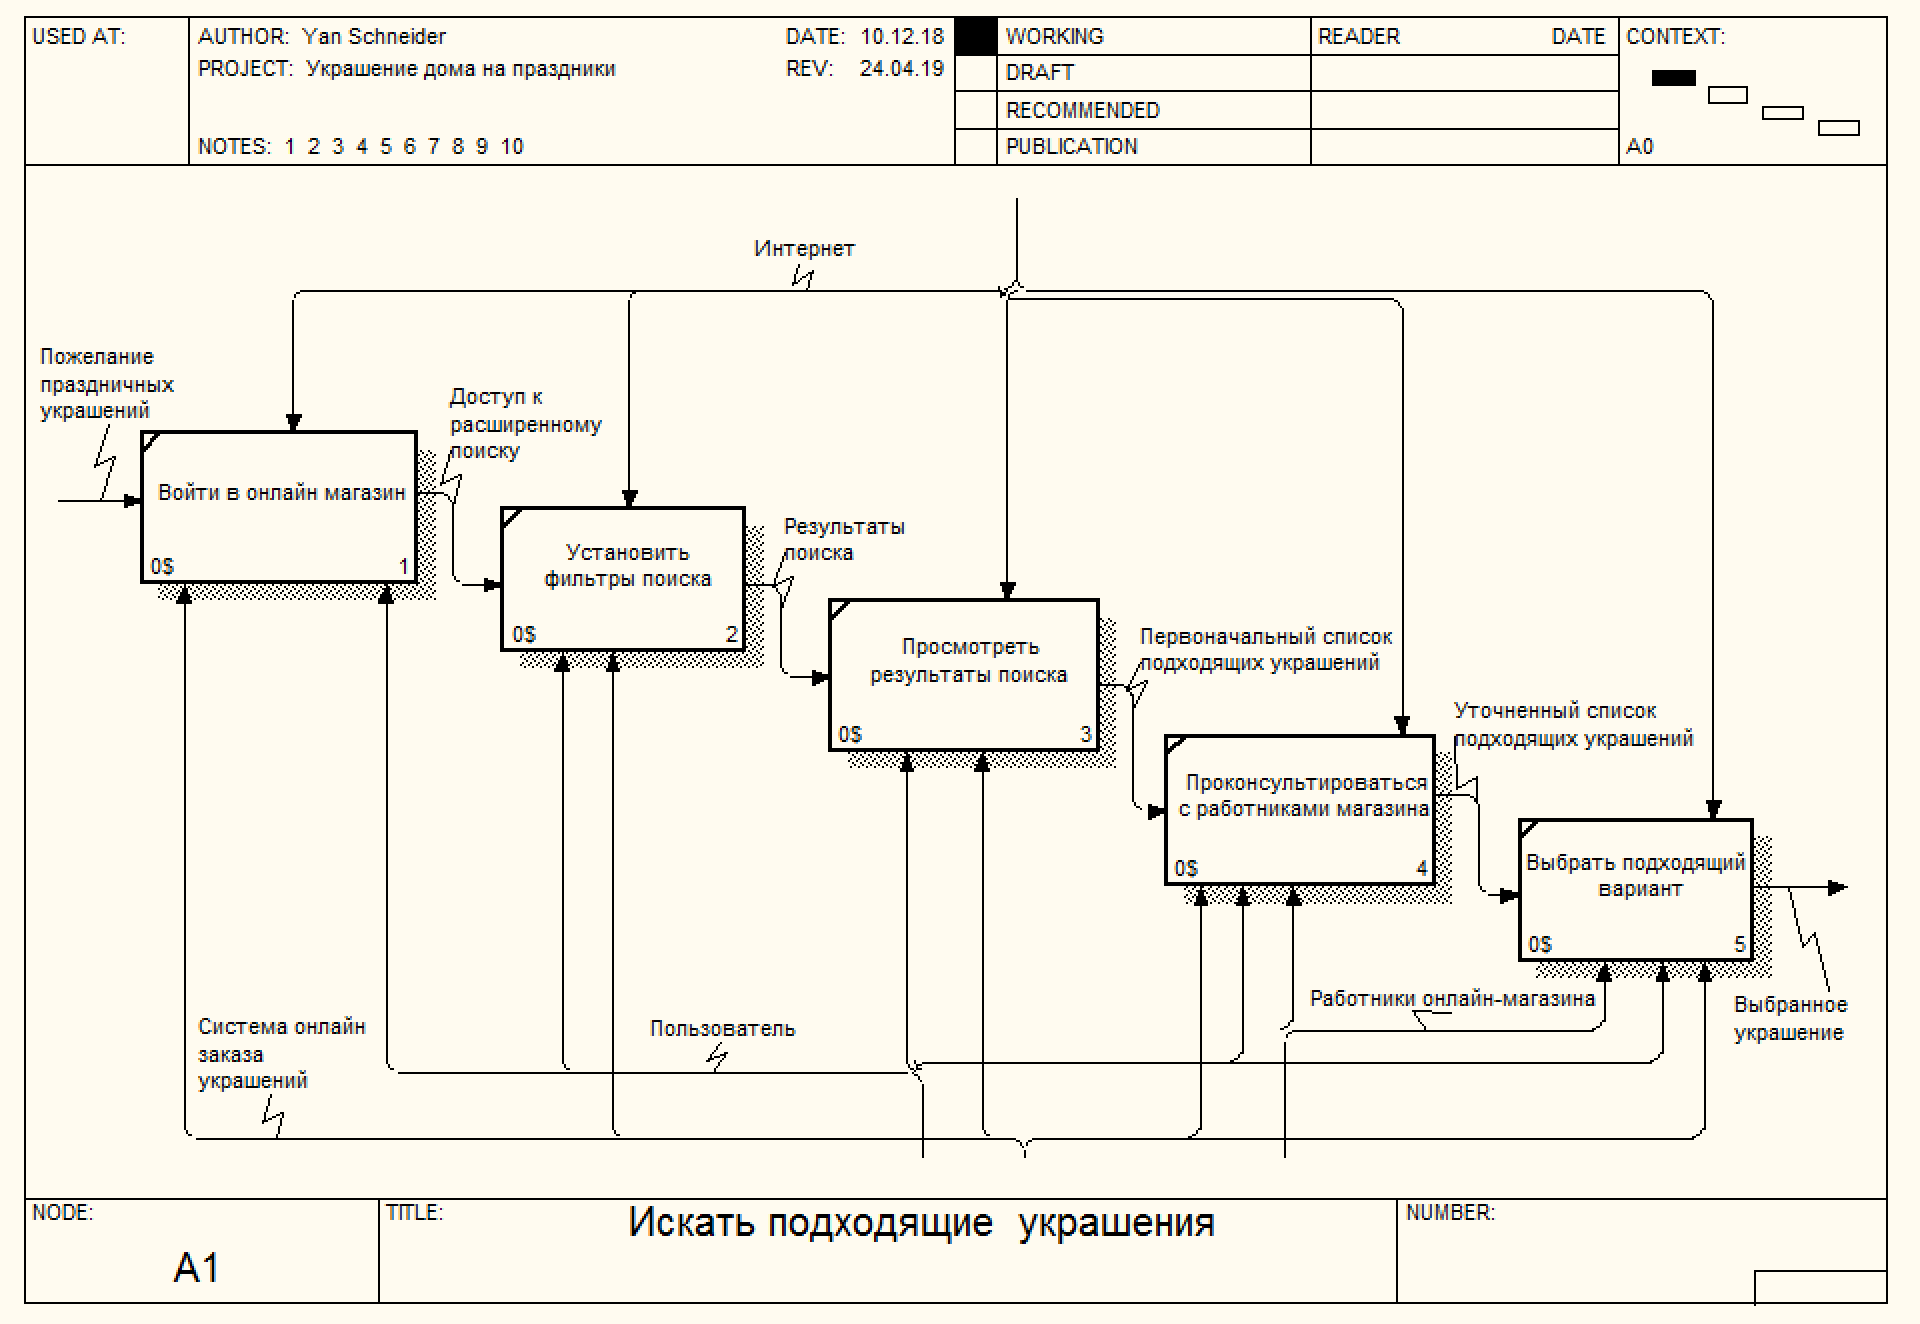
\includegraphics[scale=0.45]{figures/functionalModel/a1_search.png}
	\caption{Декомпозиция блока \enquote{Искать подходящие украшения}}
	\label{fig:analysis:functionalModel:a1_search}
\end{figure}

Второй блок представлен на рисунке~\ref{fig:analysis:functionalModel:a2_buy}. Данный блок включает в себя добавление заказа (украшения) в корзину, ввод платежной информации, ввод информации о доставке (адрес, индекс и т.д.) и оплата товара.

 ~
\begin{figure}[H]
\centering
	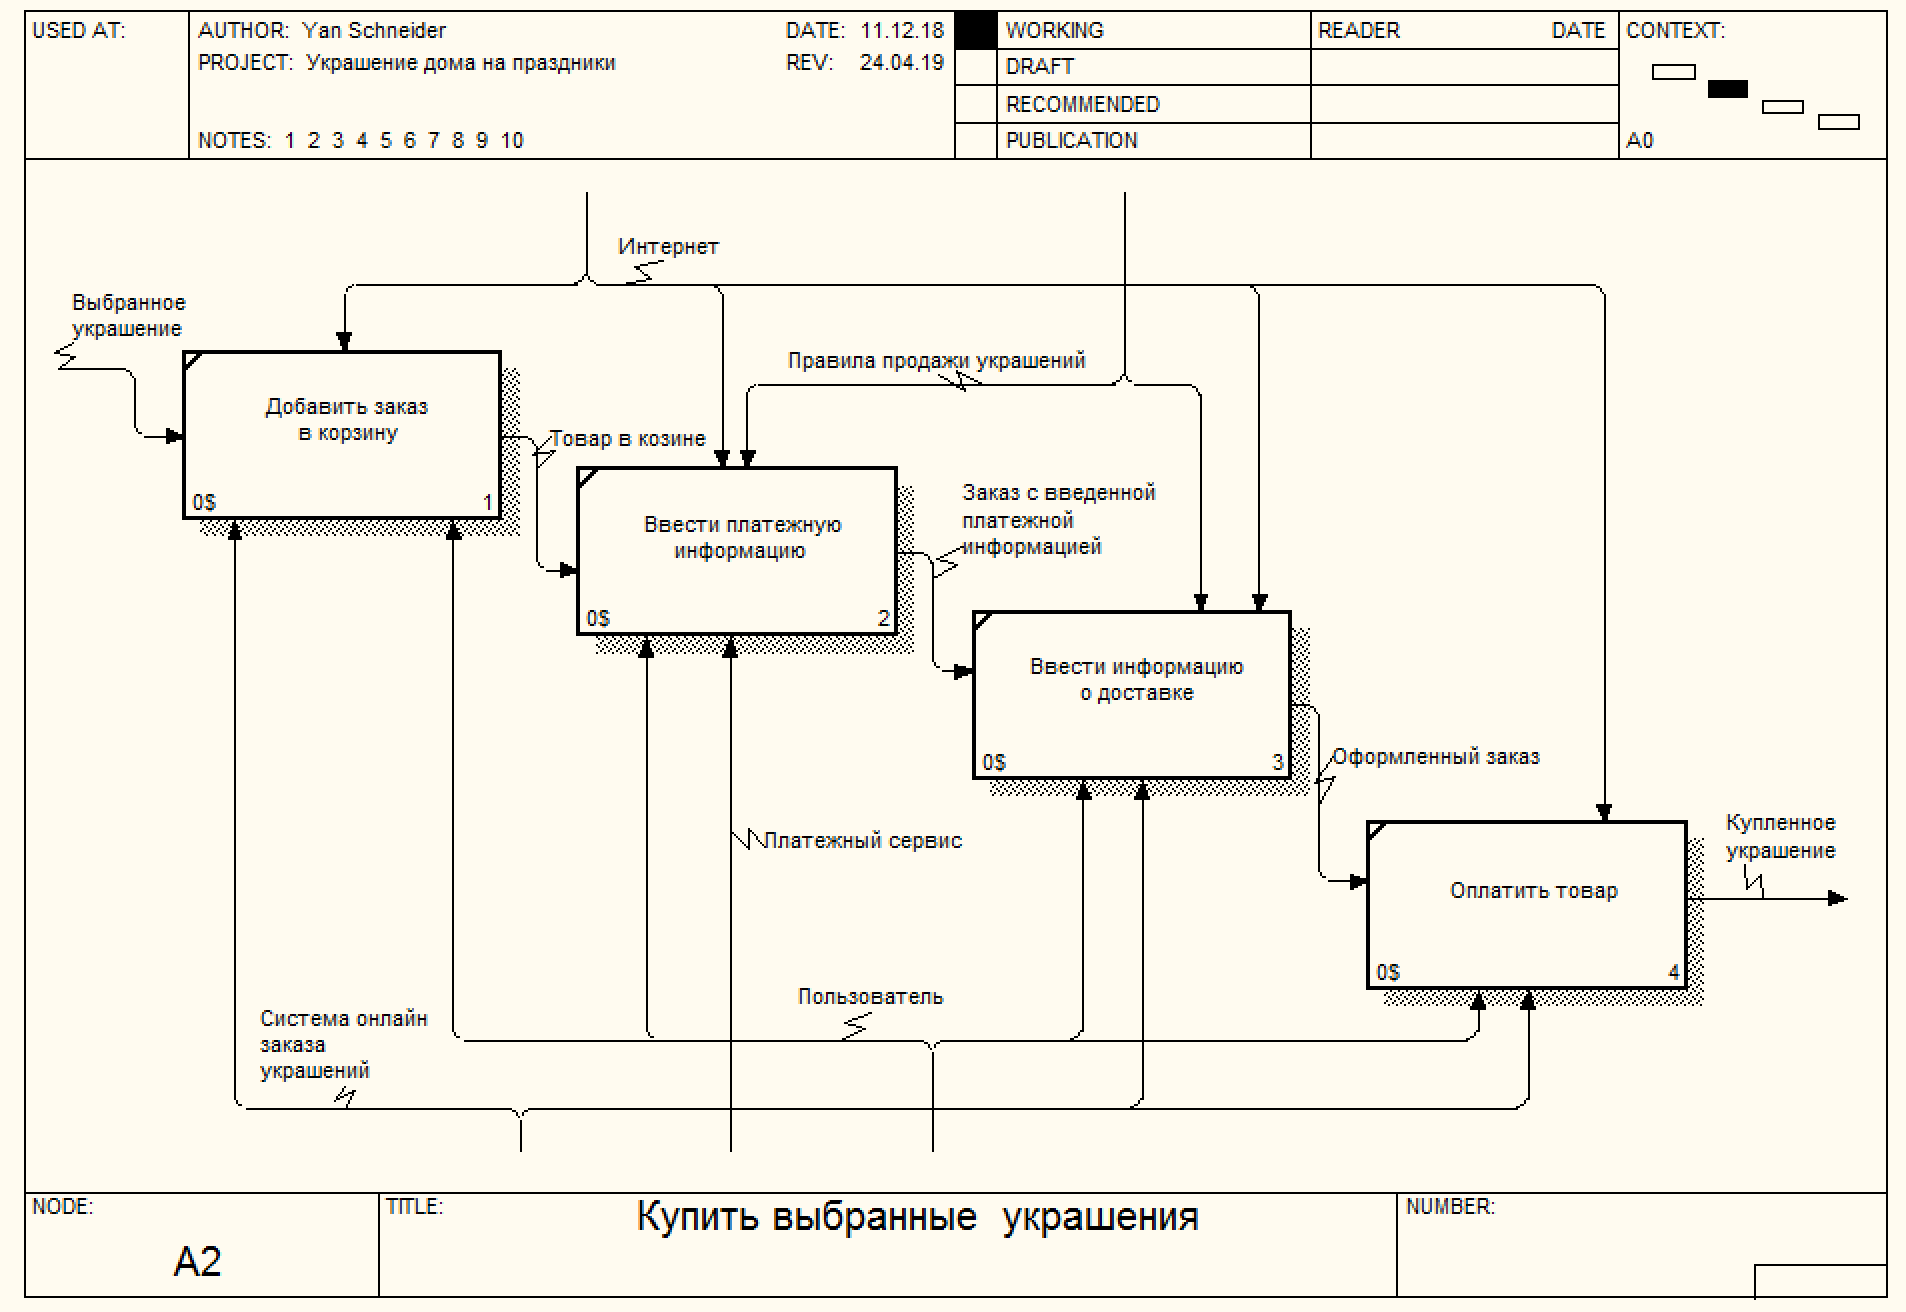
\includegraphics[scale=0.45]{figures/functionalModel/a2_buy.png}
	\caption{Декомпозиция блока \enquote{Купить выбранные украшения}}
	\label{fig:analysis:functionalModel:a2_buy}
\end{figure}

 ~
\begin{figure}[H]
\centering
	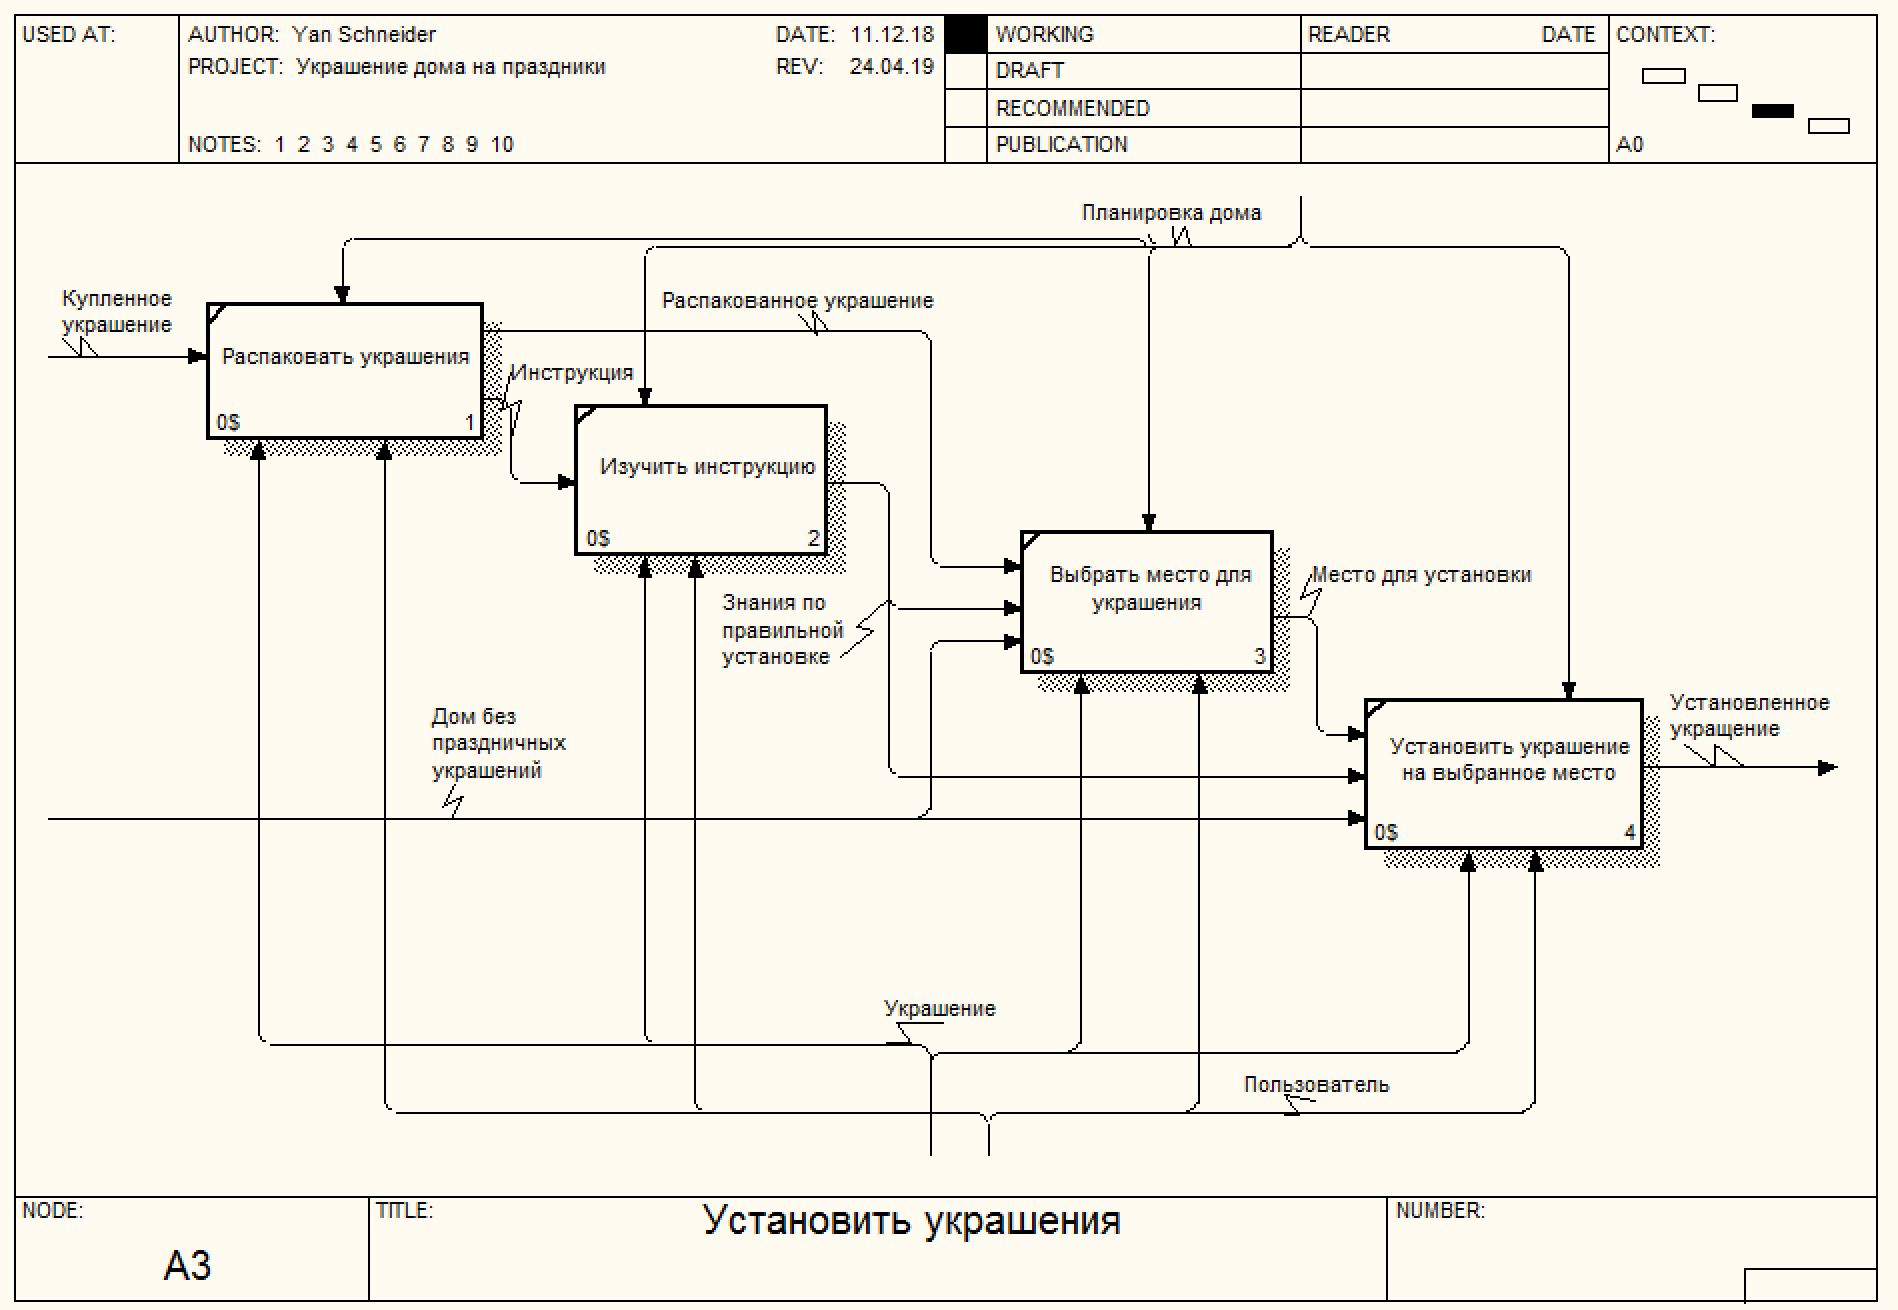
\includegraphics[scale=0.45]{figures/functionalModel/a3_install.png}
	\caption{Декомпозиция блока \enquote{Установить украшения}}
	\label{fig:analysis:functionalModel:a3_install}
\end{figure}

Третий блок (рисунок~\ref{fig:analysis:functionalModel:a3_install}):

Данный блок описывает процесс установки купленного украшения в доме. Данный процесс включает в себя распаковку украшения, чтение инструкции, выбор места для украшения и его установка.

 ~
\begin{figure}[H]
\centering
	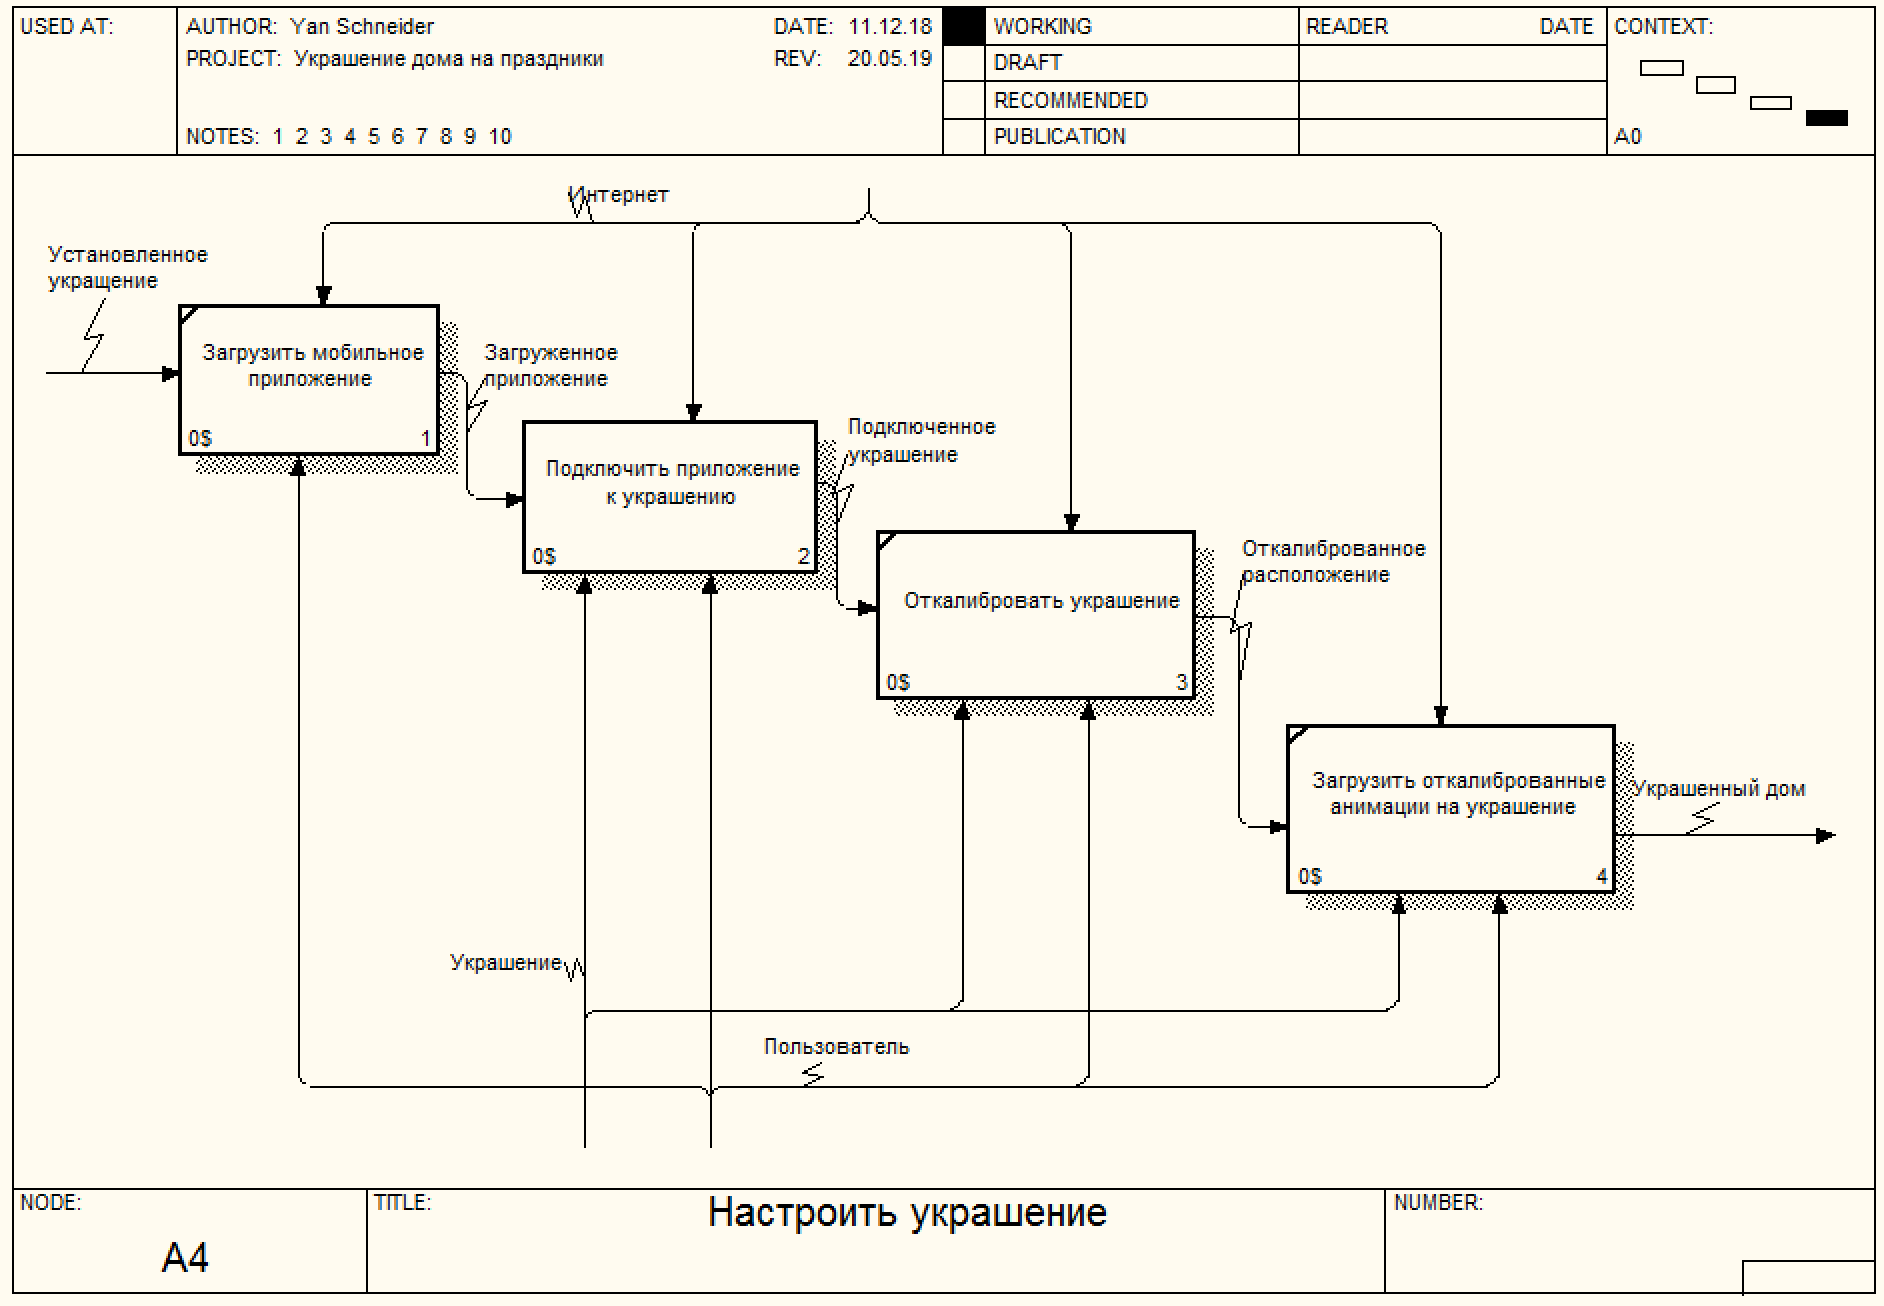
\includegraphics[scale=0.45]{figures/functionalModel/a4_settings.png}
	\caption{Декомпозиция блока \enquote{Настроить украшения}}
	\label{fig:analysis:functionalModel:a4_settings}
\end{figure}

Четвертый блок (рисунок~\ref{fig:analysis:functionalModel:a4_settings}):

Данный блок описывает процесс настройки украшений. Данный процесс включает в себя загрузку приложения для управления украшениями, подключение их к приложению, калибровку и отправку уже откалиброванных анимаций на украшения. 

~
\begin{figure}[H]
\centering
	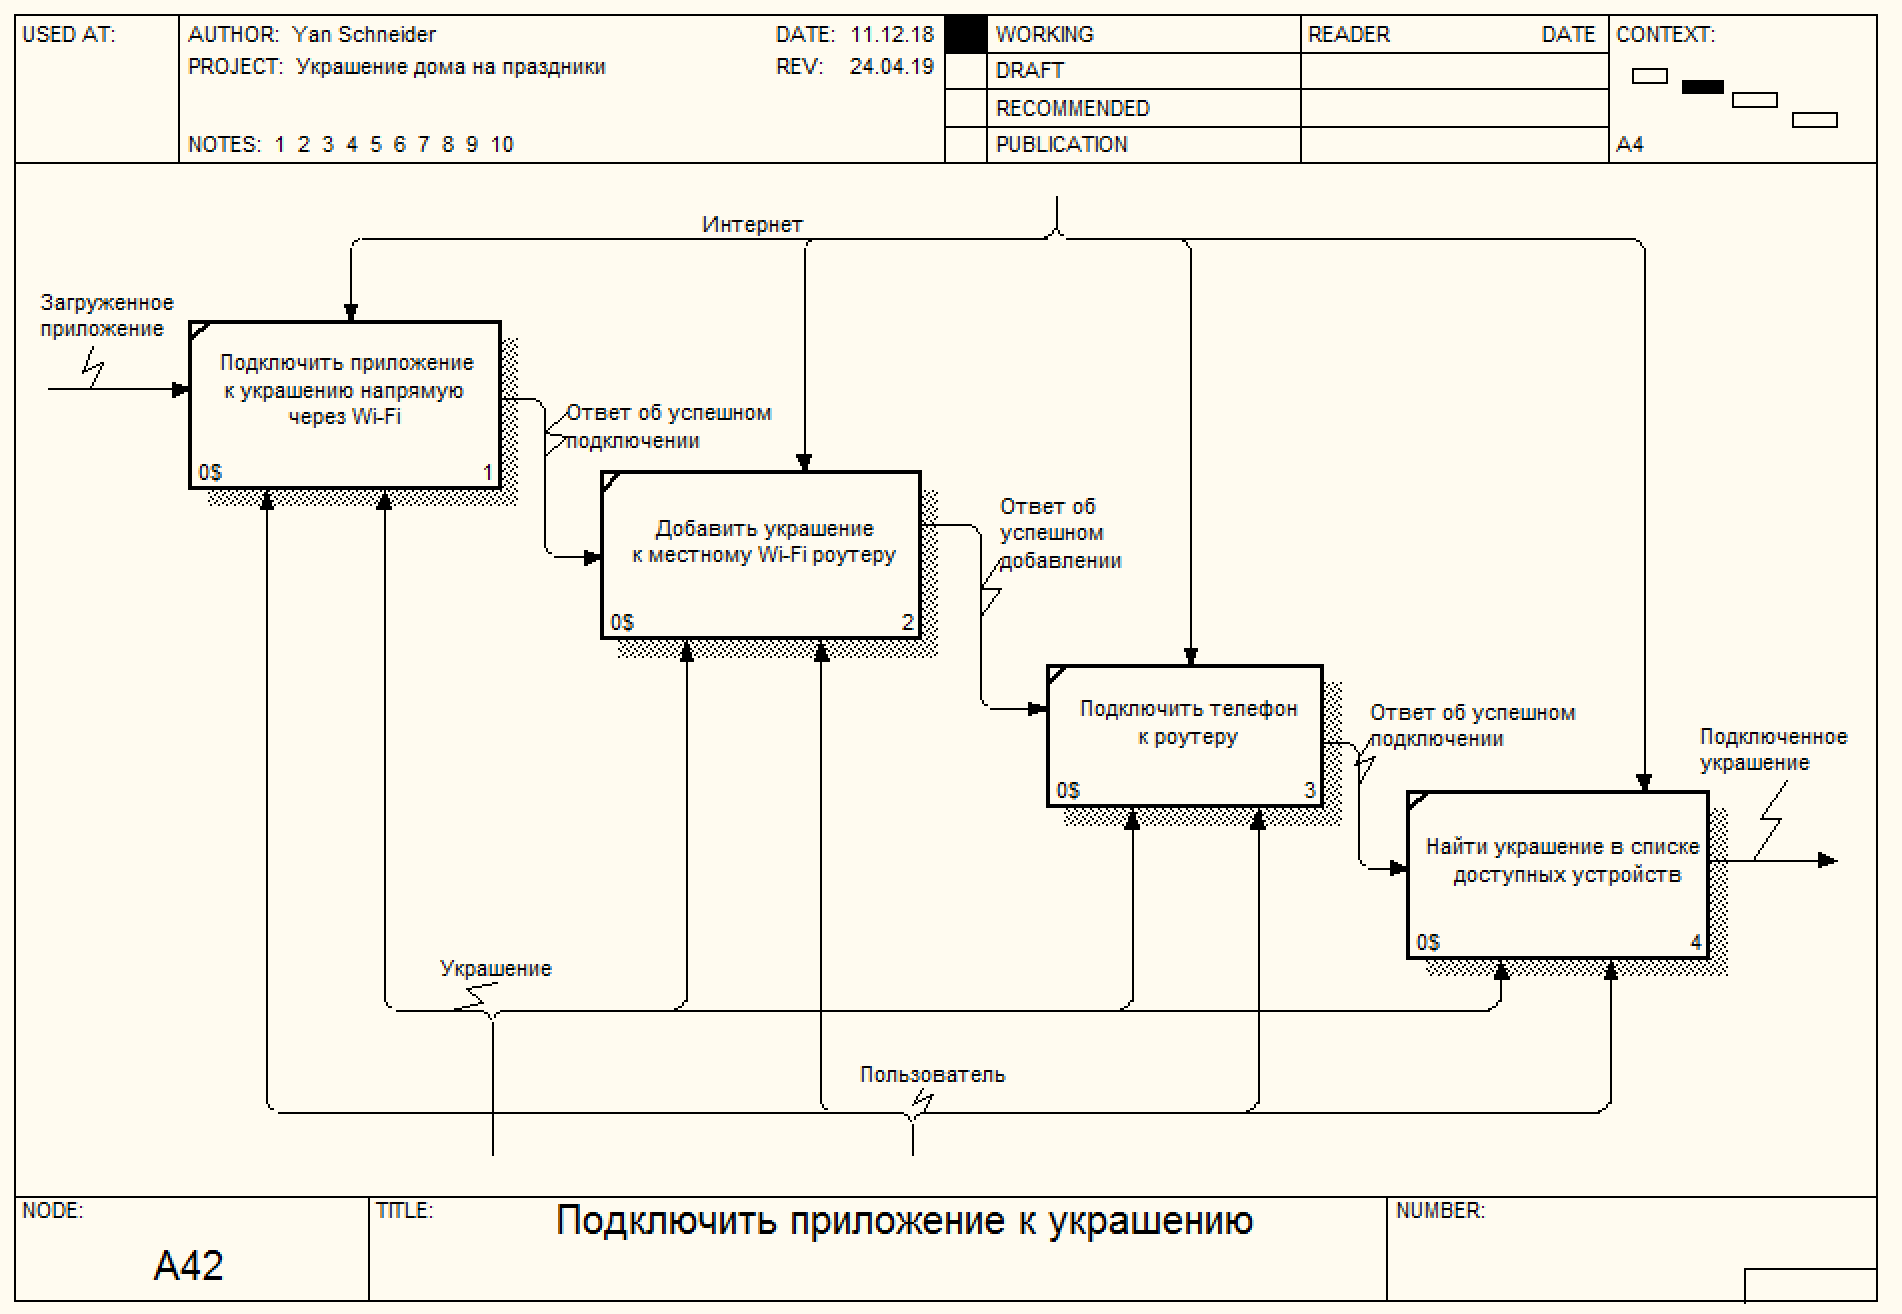
\includegraphics[scale=0.45]{figures/functionalModel/a42_connecting.png}
	\caption{Декомпозиция блока \enquote{Подключить приложение к украшению}}
	\label{fig:analysis:functionalModel:a42_connecting}
\end{figure}

Декомпозиция четвертого блока (рисунок~\ref{fig:analysis:functionalModel:a42_connecting}):

Данная декомпозиция подробнее рассматривает процесс подключения мобильного приложения к украшению (украшениям). Она разбивает данный процесс на следующие компоненты: подключение напрямую к украшению через Wi-Fi, добавление украшения к местному роутеру (ввод пароля к точке). Затем идет процес подключения телефона к роутеру. После всего следует поиск украшения в списке доступных устройств.

Итак, был исследован процесс приобретения и управления адресной светодиодной лентой. Представлена информация о компании Sampad, и роли Интернета вещей в ее деятельности. На основе результатов исследования был проведен анализ рынка Интернета вещей и исследован его прогноз на 2019 год. В результате анализа и исследования была предложена новая модель взаимодействия пользователя с адресной лентой. Новая модель включает в себя специально разработанную адресную ленту, а также мобильное приложение, с помощью которого пользователи получат возможность полноценно управлять данной лентой.
